% !TeX spellcheck = id_ID
\documentclass[a4paper,12pt]{article}
\usepackage[indonesian]{babel}
\usepackage{graphicx}
\usepackage{multirow}
\usepackage{enumitem}
\usepackage{listings}
\usepackage{wrapfig}
\usepackage[T1]{fontenc}
\usepackage{inconsolata}
\usepackage{lipsum}
\usepackage{adjustbox}


\usepackage{color}
\usepackage[table]{xcolor}
\definecolor{mygreen}{rgb}{0,0.6,0}
\definecolor{mygray}{rgb}{0.5,0.5,0.5}
\definecolor{mymauve}{rgb}{0.58,0,0.82}
\lstset{%
    language=java,
    backgroundcolor=\color{white},   % choose the background color
    basicstyle=\footnotesize,        % size of fonts used for the code
    breaklines=true,                 % automatic line breaking only at whitespace
    captionpos=b,                    % sets the caption-position to bottom
    commentstyle=\color{mygreen},    % comment style
    escapeinside={\%*}{*)},          % if you want to add LaTeX within your code
    keywordstyle=\color{blue},       % keyword style
    stringstyle=\color{mymauve},     % string literal style
}

\graphicspath{ {./img/} }
\begin{document}
\title{ {\Large Tugas}\\ Algoritma dan Pemrograman Lanjut\\{\Large Pertemuan 1}}

\author{Aldzikri Dwijayanto Prathama 
	\\195410189
	\\Informatika}
\makeatletter
\begin{titlepage}
	\begin{center}
		{\huge \bfseries \@title }\\[14ex]
		
\includegraphics[scale=.8]{logo}\\[4ex]
		{\large \@author}\\[12ex]
		{\large \bfseries {SEKOLAH TINGGI MANAJEMEN INFORMATIKA DAN KOMPUTER
				AKAKOM YOGYAKARTA}}
	\end{center}


%{\large \@date} 
\end{titlepage}
\makeatother
%\maketitle
\newpage

\section{Latihan}
\begin{lstlisting}[frame=single]
import java.util.Scanner;
public class Latihan{
    public static void main (String arg[]){
        Scanner in = new Scanner(System.in);
        int jawab;
        System.out.print("1.Mobil 2.Motor = ");
        jawab= in.nextInt();
        switch(jawab)
        {
            case 1:
            System.out.print("1.Honda 2.Suzuki = ");
            jawab = in.nextInt();
            switch(jawab)
            {
                case 1:
                System.out.print("1.Jazz 2.Brio 3.Mobilio = ");
                jawab=in.nextInt();
                switch(jawab)
                {
                    case 1:
                    System.out.println("Jazz = 170jt");
                    break;
                    case 2:
                    System.out.println("Brio = 120jt");
                    break;
                    case 3:
                    System.out.println("Mobilio = 170jt");
                    break;
                }
                break;
                case 2:
                System.out.print("1.APV 2.Swift 3.Ertiga = ");
                jawab=in.nextInt();
                switch(jawab)
                {
                    case 1:
                    System.out.println("APV = 180jt");
                    break;
                    case 2:
                    System.out.println("Swift = 155jt");
                    break;
                    case 3:
                    System.out.println("Ertiga = 160jt");
                    break;
                }
                break;
            }
            break;
            case 2:
            System.out.print("1.Honda 2.Yamaha = ");
            jawab = in.nextInt();
            switch(jawab)
            {
                case 1:
                System.out.print("1.Vario 2.Supra = ");
                jawab=in.nextInt();
                switch(jawab)
                {
                    case 1:
                    System.out.println("Vario = 15jt");
                    break;
                    case 2:
                    System.out.println("Supra = 12jt");
                    break;
                }
                break;
                case 2:
                System.out.print("1.Mio 2.Vixion = ");
                jawab=in.nextInt();
                switch(jawab)
                {
                    case 1:
                    System.out.println("Mio = 14jt");
                    break;
                    case 2:
                    System.out.println("Vixion = 20jt");
                    break;
                }
                break;
            }
            break;
        }
    }
}
\end{lstlisting}
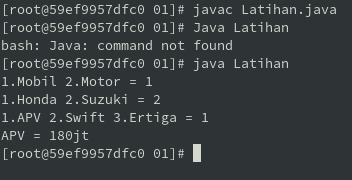
\includegraphics{Latihan.png}

\section{Tugas}
\begin{lstlisting}[frame=single]
import java.util.Scanner;
public class Pemilu{
    public static void main (String arg[]){
        Scanner in = new Scanner(System.in);
        int jawab;
        System.out.print("Berapa umur anda? = ");
        jawab=in.nextInt();
        if(jawab >= 17)
        {
            System.out.println("Apakah anda warga negara Indonesia? 1.Ya 2.Tidak");
            jawab=in.nextInt();
            if (jawab == 1) 
            {
                System.out.println("Apakah anda TNI aktif? 1.Ya 2.Tidak");
                jawab=in.nextInt();
                if (jawab ==2) 
                {
                    System.out.println("Anda berhak mengikuti pemilu");
                }
                else
                {
                    System.out.println("Anda tidak berhak mengikuti pemilu");
                }
            }
            else
            {
            System.out.println("Anda tidak berhak mengikuti pemilu");
            }
        }
        else
        {
            System.out.println("Anda tidak berhak mengikuti pemilu");
        }
    }
}
\end{lstlisting}
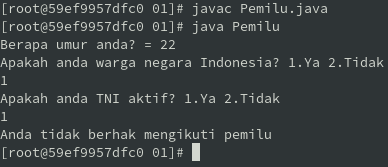
\includegraphics{Pemilu_program.png}

\end{document}
